\documentclass[15pt]{article}
\usepackage{amsmath} %% to give math notations
\usepackage{graphicx} %% to include pictures
\usepackage{float} %% to fix the locations of pictures

\title{IE 534 Homework 6 Report}
\author{Hanwen Hu}

\begin{document}
\maketitle

This homework asks to first train the Discriminator without Generator, then train both Discriminator and Generator at the same time. Then, it's required that some pictures should be shown in order to show the effectiveness of GAN techniques.

\section{Hyperparameter Settings and Time Cost}
For the first training without Generator, the process runs 51 epochs in total, costing 118 minutes. ADAM is applied during training, and the original learning rate is given as 1e-4. \\
Input images are shuffled, then divided into mini batches, with batch size as 128. Several types of data augmentation are implemented on train set, including random horizontal flip, random resized crop, random color jitter and normalization with mean 0.5 and sd 0.5 on all channels. Center crop and normalization is also implemented on the test set.\\
\\
For the second training with Generator, the training process runs 200 epochs in total, costing 46 hours and 51 minutes. ADAM is applied during training, and the original learning rate is given as 1e-4.\\
Input images are shuffled, then divided into mini batches, with batch size as 100. Several types of data augmentation are implemented on train set, exactly the same as the first training process. Center crop and normalization is also implemented on the test set.\\

\section{Accuracy Graph}
For the first Discriminator trained without Generator, the train accuracy achieves the maximum of 98.20\% at the 50th epoch, and test accuracy achieves maximum of 88.84\% at the 50th epoch;\\
For the second Discriminator trained with Generator, the train accuracy achieves the maximum of 94.12\% at the 195th epoch, and test accuracy achieves maximum of 86.72\% at the 147th epoch, but then oscillating around 85\% and 86\%.
\begin{figure}
\centering
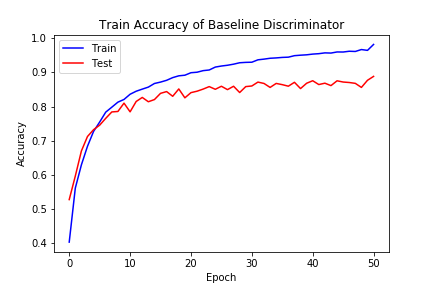
\includegraphics[width=\textwidth]{../Baseline_Accuracy_Plot}
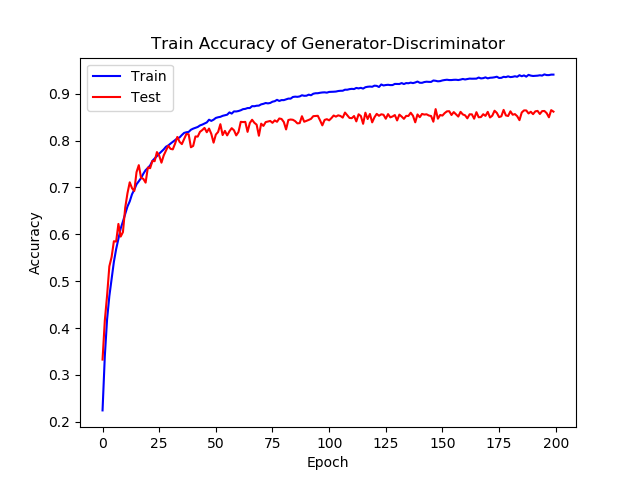
\includegraphics[width=\textwidth]{../Gen_Disc_Accuracy_Plot}
\caption{Accuracy graph of Discriminator trained without(Up) and with(Down) Generator}
\end{figure}

\section{Result printing}
\subsection{Generated images on different epochs}

\begin{figure}[H]
\centering
\includegraphics[width=\textwidth]{../Plots/output_039}
\caption{Train Loss graph of Epoch 40}
\end{figure}
\begin{figure}[H]
\centering
\includegraphics[width=\textwidth]{../Plots/output_079}
\caption{Train Loss graph of Epoch 80}
\end{figure}
\begin{figure}[H]
\centering
\includegraphics[width=\textwidth]{../Plots/output_119}
\caption{Train Loss graph of Epoch 120}
\end{figure}
\begin{figure}[H]
\centering
\includegraphics[width=\textwidth]{../Plots/output_159}
\caption{Train Loss graph of Epoch 160}
\end{figure}
\begin{figure}[H]
\centering
\includegraphics[width=\textwidth]{../Plots/output_199}
\caption{Train Loss graph of Epoch 200}
\end{figure}

\subsection{Fake images that are wrongly classified}
\begin{figure}[H]
\centering
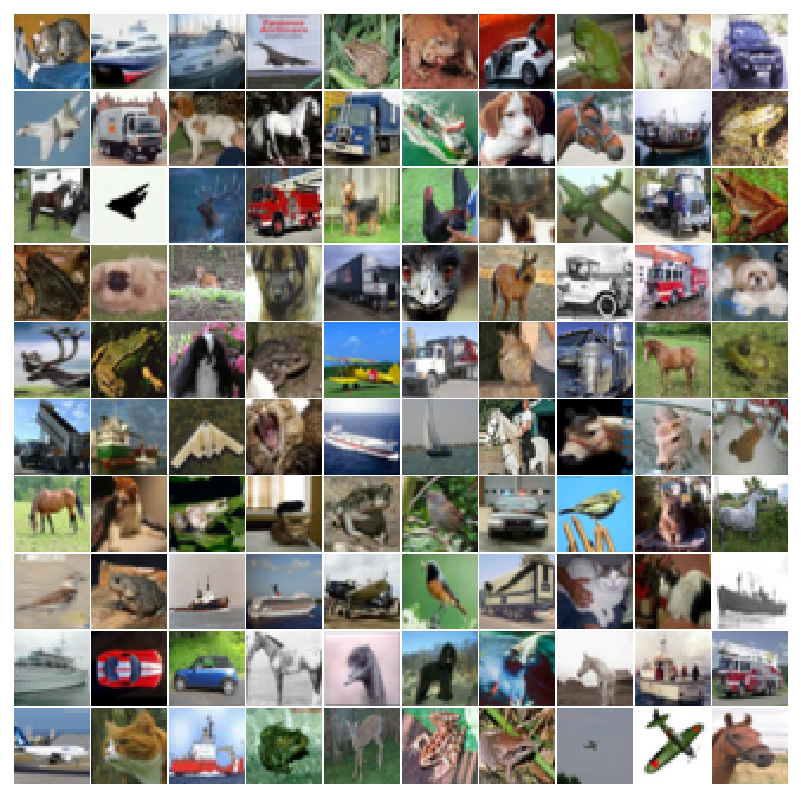
\includegraphics[width=\textwidth]{../Visualization/real_images}
\caption{A batch of real images}
\end{figure}

\begin{figure}[H]
\centering
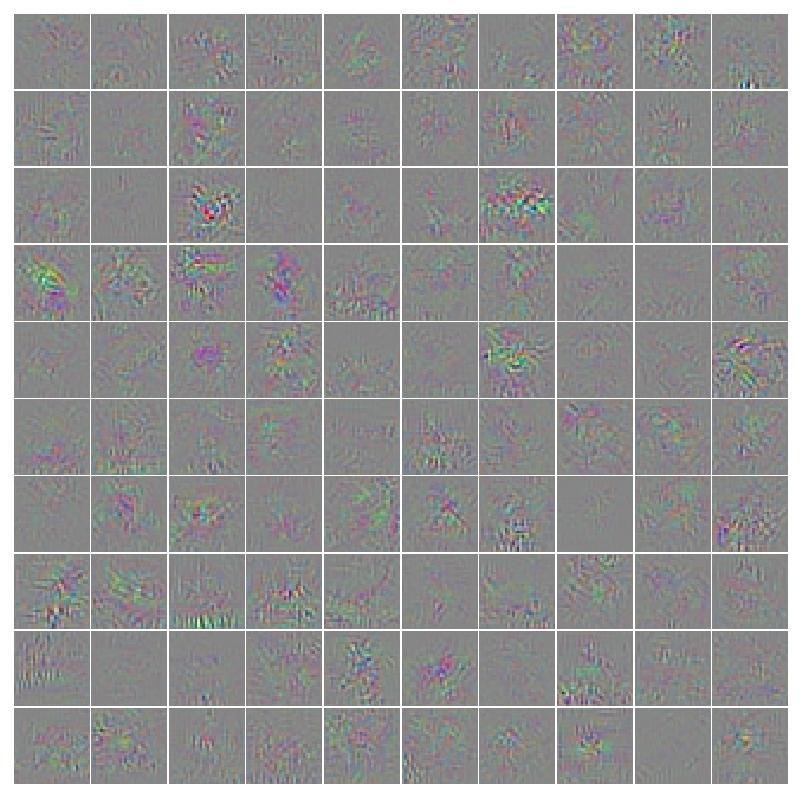
\includegraphics[width=\textwidth]{../Visualization/gradient_image}
\caption{Corresponding gradients}
\end{figure}

\begin{figure}[H]
\centering
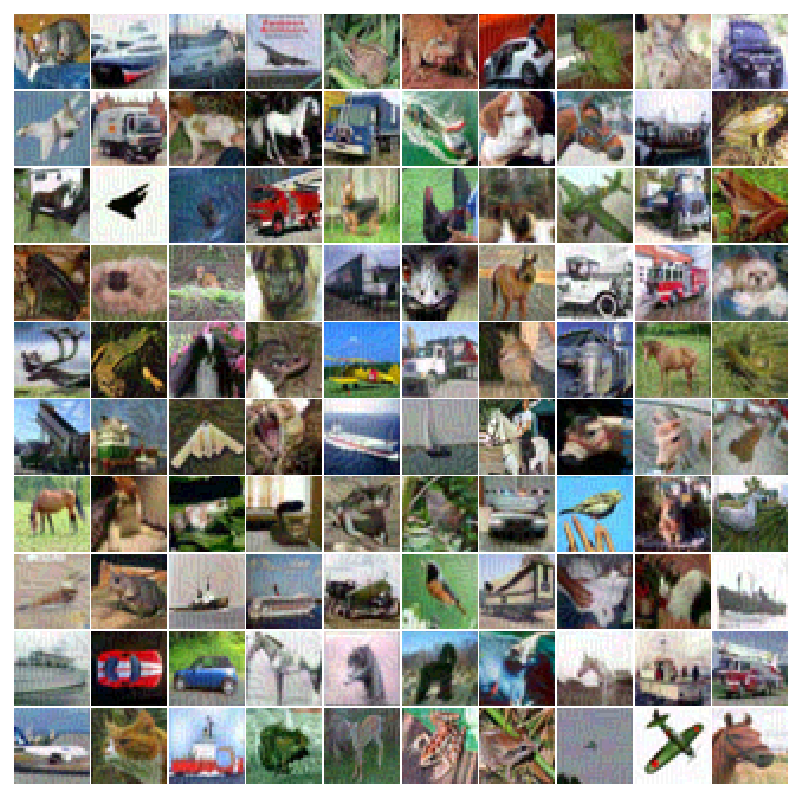
\includegraphics[width=\textwidth]{../Visualization/jittered_images}
\caption{Corresponding modified images}
\end{figure}

\subsection{Synthetic images maximizing classification output}

\begin{figure}[H]
\centering
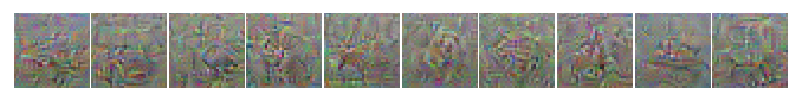
\includegraphics[width=\textwidth]{../Visualization/max_class_no_generator}
\caption{Synthetic images maximizing class output for discriminator trained without the generator}
\end{figure}

\begin{figure}[H]
\centering
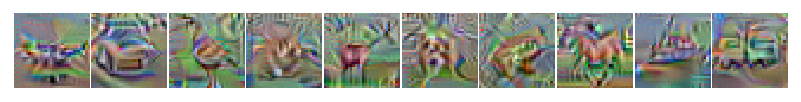
\includegraphics[width=\textwidth]{../Visualization/max_class_with_generator}
\caption{Synthetic images maximizing class output for discriminator trained with the generator}
\end{figure}

\end{document}
